\subsection{Primo tutorial: gestione dei tasks}
Come in Maven ci sono i goals, in Gradle ci sono i task, ognuno dei quali ha il suo scopo definito nella sua implementazione. Gradle si basa su build multi-task, il primo esempio si basa sulla comprensione del funzionamento delle build Maven.

\subsubsection{Task e Task dependency}
Creiamo una cartella in cui inserire il file di configurazione della build Gradle chiamato build.gradle e modifichiamo il suo contenuto usando un editor di testo:
\begin{verbatim}
task compile {
    doLast {
        println 'compiling source'
    }
}

task compileTest(dependsOn: compile) {
    doLast {
        println 'compiling unit tests'
    }
}

task test(dependsOn: [compile, compileTest]) {
    doLast {
        println 'running unit tests'
    }
}

task dist(dependsOn: [compile, test]) {
    doLast {
        println 'building the distribution'
    }
} \end{verbatim}
a questo punto dovremmo avere una cosa di questo tipo:
\begin{figure}[H]
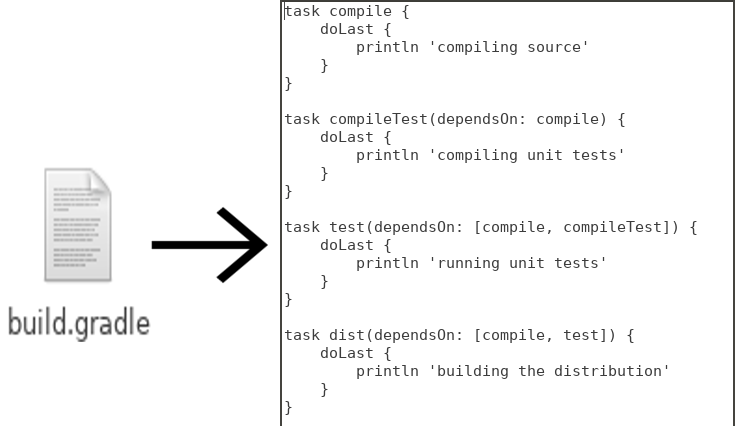
\includegraphics[scale=0.40]{Tutorial/first/gradleexamplefirst.png}
\end{figure} 
abbiamo creato un albero di dipendenze tra tasks di questo tipo:
\label{taskdip}
\begin{figure}[H]
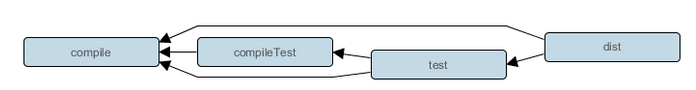
\includegraphics[scale=0.70]{Tutorial/first/taskdipendence.png}
\end{figure}
è possibile fare diverse build con questa configurazione:
\begin{itemize}
    \item \begin{verbatim} $ gradle compile \end{verbatim}
    \item \begin{verbatim} $ gradle compileTest \end{verbatim}
    \item \begin{verbatim} $ gradle test \end{verbatim}
    \item \begin{verbatim} $ gradle dist \end{verbatim}
    \item una combinazione qualunque di 2 o più task.
\end{itemize}
Possiamo notare che anche se eseguiamo la build: 
\begin{verbatim}
    $ gradle compile test \end{verbatim}
il task \textbf{compile} verrà eseguito solo una volta:
\begin{verbatim}
> Task :compile 
compiling source

> Task :compileTest 
compiling unit tests

> Task :test 
running unit tests


BUILD SUCCESSFUL in 0s
3 actionable tasks: 3 executed \end{verbatim}

\subsubsection{Escludere task da una build}
È possibile escludere un task di una build, aggiungendo come argomento il task da escludere preceduto da -x:
\begin{verbatim}
    $ gradle <task_da_eseguire> -x <task_da_escludere> \end{verbatim}
questo viene usato al fine di eliminare un task inutile per lo scopo della build che abbiamo intenzione di eseguire. Riprendendo l'esempio del paragrafo precedente se andiamo ad eseguire la build:
\begin{verbatim}
    $ gradle dist \end{verbatim}
vediamo che vengono eseguiti tutti i tasks, compresi i tasks \textbf{test} e \textbf{compileTest}, supponendo di voler fare solo la build del sorgente possiamo scrivere:
\begin{verbatim}
    $ gradle dist -x test
\end{verbatim}
l'output risultante sarà:
\begin{verbatim}
> Task :compile 
compiling source

> Task :dist 
building the distribution


BUILD SUCCESSFUL in 0s
2 actionable tasks: 2 executed \end{verbatim}
Il task \textbf{compileTest} non viene eseguito perchè dipendenza di \textbf{test}, ma non di \textbf{dist} (vedi pag. \pageref{taskdip}), escludendo il primo quindi non è necessario eseguire il task \textbf{compileTest}. Nel file di configurazione della build è possibile inserire anche un descrizione inserendo in testa al file build.gradle la seguente riga:
\begin{verbatim}
    description = 'Descrizione' \end{verbatim}
Questo è importante per progetti multi-builds consentendo di avere una descrizione di ogni singola build.

\subsubsection{Abbreviazione del nome del task} è possibile abbreviare il nome del task da eseguire stando però attenti ad identificare unicamente il task che vogliamo eseguire, per esempio se volessi eseguire il task \textbf{compileTest} potrei farlo semplicemente con il comando:
\begin{verbatim}
    $ gradle comTes \end{verbatim}
considerando i task creati precedentemente notiamo che il task è univocamente identificato.

\subsubsection{Selezionare la build da eseguire} consideriamo che esista in una subdirectory chiamata subdir una build chiamata subbild.gradle, partendo dalla directory root è possibile eseguire questa build eseguendo il comando:
\begin{verbatim}
    $ gradle -b subdir/subbuild.gradle <task_da_eseguire> \end{verbatim}
è possibile anche indicare direttamente la project directory da usare, nel nostro caso indicheremo subdir:
\begin{verbatim}
    $ gradle -p subdir  \end{verbatim}

\subsubsection{Forzare l'esecuzione di un task} a causa della Gradle cache è possibile che un task o più di uno non vengano eseguiti perchè marcati come UP-TO-DATE (anche se dalla versione Gradle 4.0 non viene più mostrato in output), in questo caso è possibile forzarne l'esecuzione con:
\begin{verbatim}
    $ gradle --rerun-tasks <tasks_da_eseguire> \end{verbatim}

\subsubsection{Ottenere informazioni generali} come già detto precedentemente nel caso di progetti multi-builds è necessario avere una descrizione di ogni file di configurazione della build, per ottenere le informazioni sul progetto corrispondente alla build è possibile eseguire il task \texttt{projects}:
\begin{verbatim}
    $ gradle projects \end{verbatim}

\subsubsection{Ottenere informazioni sui tasks} è possibile ricavare una lista dei tasks default eseguendo la build del task \texttt{tasks}:
\begin{verbatim}
    $ gradle tasks \end{verbatim}
possiamo notare che l'output non mostra tutti i task, ma solo quelli predefiniti:
\begin{verbatim}
> Task :tasks 

------------------------------------------------------------
All tasks runnable from root project - Descrizione
------------------------------------------------------------

Build Setup tasks
-----------------
init - Initializes a new Gradle build.
wrapper - Generates Gradle wrapper files.

Help tasks
----------
buildEnvironment - Displays all buildscript dependencies declared in root project 'first'.
components - Displays the components produced by root project 'first'. [incubating]
dependencies - Displays all dependencies declared in root project 'first'.
dependencyInsight - Displays the insight into a specific dependency in root project 'first'.
dependentComponents - Displays the dependent components of components in root project 'first'. [incubating]
help - Displays a help message.
model - Displays the configuration model of root project 'first'. [incubating]
projects - Displays the sub-projects of root project 'first'.
properties - Displays the properties of root project 'first'.
tasks - Displays the tasks runnable from root project 'first'.

To see all tasks and more detail, run gradle tasks --all

To see more detail about a task, run gradle help --task <task>


BUILD SUCCESSFUL in 0s
1 actionable task: 1 executed \end{verbatim}
come dice l'output, per visualizzare la lista di tutti i tasks è necessario eseguire la build del task \texttt{tasks} con argomento --all:
\begin{verbatim}
    $ gradle tasks --all \end{verbatim}
    il risultato sarà molto più specifico rispetto al precedente. Possiamo notare che a differenza degli altri tasks quelli che abbiamo creato noi sono sprovvisti di una descrizione, per aggiungerla basterà inserire un campo \texttt{description} all'interno della definizione del task:
    \begin{verbatim}
task dist(dependsOn: [compile, test]) {
    description = 'Build distribution'
    doLast {
        println 'building the distribution'
    }
} \end{verbatim}
rieseguendo il comando sopra otterremo una descrizione anche per il \texttt{dist}. Per ottenere informazioni più specifiche è possibile usare la build del task help seguito da --task e il nome del task:
\begin{verbatim}
    $ gradle help --task <task> \end{verbatim}
quello che vedremo sarà un riepilogo generale del task.